\section*{Analyse} % (fold)
\label{sec:analyse}

% Wie haben wir die Daten gewonnen ?
% Autohotkey ...
% java -jar loader.jar gui > data.txt

%Denk an die Fragestellung die ich aufgestellt habe und sag in wie weit die Ergebnisse auf eine reale Arbeitsumgebung anwendbar sind (nur bedingt ...)

% 9. Dezille heißt, dass 90% der Werte unterhalb dieses Wertes liegen und 10% drüber -> Fragestellung



\begin{figure}[ht]
  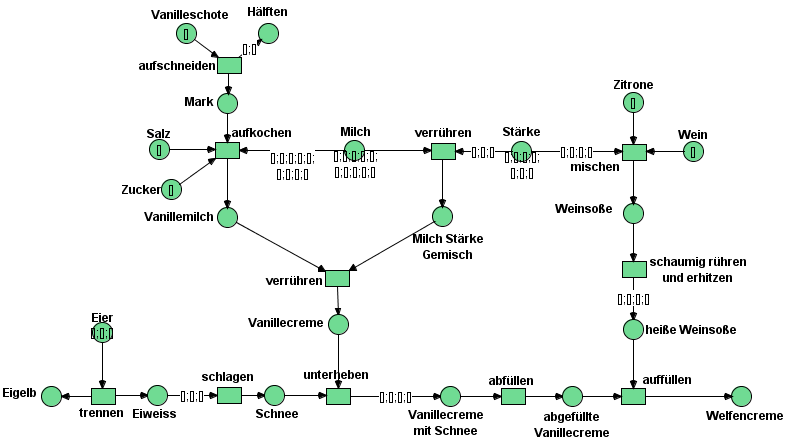
\includegraphics[width=1\textwidth]{pics/sim.png}
  \caption{Histogramm: Die Simulation des Petrinetzes mit verschiedener Anzahl Köchen, gepunktet der korrespondierende Median, dunkel gestrichelt 9. Dezille}
  \label{pic:sim}
\end{figure}